\documentclass {report}
\usepackage[utf8]{inputenc}
\usepackage{polyglossia}
\usepackage{graphicx}
\usepackage{fancyvrb}

\usepackage{geometry}
 \geometry{
 a4paper,
 total={170mm,257mm},
 left=10mm,
 top=20mm,
 }

\title{Elektrisku shēmu modelēšana}
\author{Diana Dгplevska}
\date{2019. 13. marts}

\begin{document}

\maketitle
\chapter{Teorētiskā daļa}
\section{Ķēdes aprēķins}

\begin{center}
\small\addtolength{\tabcolsep}{10pt}
\begin{tabular}{|c|c|}
    \hline \multicolumn{2}{|c|}{Tabula:} \\
\hline
R1 & 7Ω\\
\hline
R2 & 9Ω\\
\hline
V1 & 36.8V\\
\hline
$U_{R1}$ & 16.1V\\
\hline
$U_{R2}$ & 20.7V\\
\hline
\end{tabular}
\end{center}
\chapter{Praktiskā daļa}
\section{Darbs ar gEDA programmām}
\subsection{Darbs ar gschem}
\rotatebox{-90}{\includegraphics[width=15cm,height=15cm,keepaspectratio]{01.ps}}\\
\subsection{Darbs ar gnetlist}
\VerbatimInput{01.net} \\
\begin{center}
    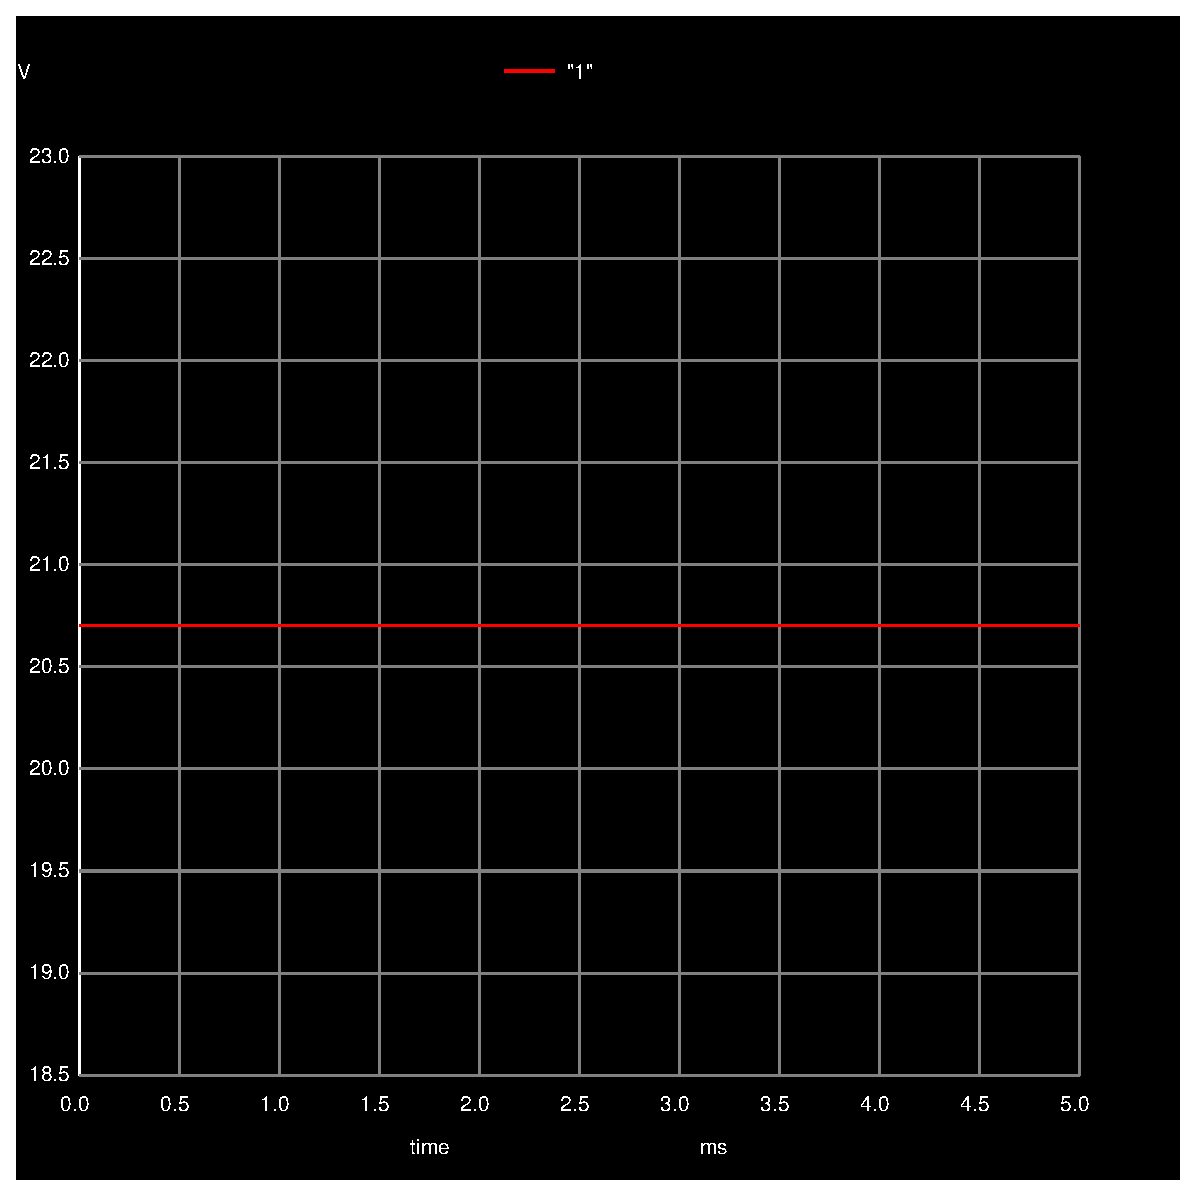
\includegraphics[width=12cm,height=12cm,keepaspectratio]{011.ps} \textit{1.attēls} \\
    \includegraphics[width=12cm,height=12cm,keepaspectratio]{022.ps} \textit{2.attēls} \\
\end{center}
\section{Darbs ar QUCS programmām}
\VerbatimInput{02.sch}
\textbf{Līdzstrāvas simulācijas grafiks:}
\rotatebox{-90}{\includegraphics[width=30cm,height=30cm,keepaspectratio]{result2.ps}}\\
\textbf{Sweep simulācijas līdzstrāvas grafiks un tabula:}
\rotatebox{-90}{\includegraphics[width=80cm,height=50cm,keepaspectratio]{result.ps}}\\

\end{document}